\documentclass[11pt]{article}
\usepackage[letterpaper, margin=1.5cm]{geometry}
\usepackage[utf8]{inputenc}
\usepackage{graphicx}
%\usepackage[uft8]{inputenc}
\usepackage{hyperref}
\usepackage{color}
\usepackage{array}
\usepackage{multirow}
\usepackage{amsmath}
\usepackage{booktabs}
\usepackage{longtable}
\usepackage{subcaption}


\newcommand{\CAVH}[1]{\begingroup\color{red}#1\endgroup}

%opening
\title{Non-protein-coding RNAs as a regulators of development in tunicates}
\author{Cristian Velandia}

\begin{document}

\maketitle

%\begin{abstract}
%\end{abstract}

\section*{miRNA families origin and evolutionary perspective}
\subsection*{miRNAs in clusters}

One of the most interesting aspects about the patterns of genomic locations of miRNAs is to known whether those loci are randomly distributed throughout the genome as single copies or if they are arranged on consecutive locations or in tandem copies clustered to be expressed from polycistronic primary precursors or to be transcribed independently. Interestingly in \textit{O. dioca} miRNAs are located in the antisense orientations of protein-coding gene and immediately downstream of its corresponding 3’ UTR region or even more in the sense strand of introns \cite{Fu2008}. Nevertheless, after those conspicuous distributions some clusters have been also identified in \textit{O. dioca}. For instance four miRNAs, miR-1490a, miR-1493, miR-1497d, and miR-1504, are reported by \cite{Fu2008} to be presented as two copies, and miR-1497d-1 and miR-1497d-2 are included in the large miR-1497 cluster. See the current structure of this cluster in Table \ref{tab:detailBigClusters} although only one copy for the  miR-1497 has been reported for \textit{C. instestinalis} located in an intergenic region \cite{Fu2008}, \cite{Hendrix2010} and one in \textit{C. savigny} overlapped in an intron \cite{Fu2008}. By testing real time PCR co-expression of some miRNAs, their host and adjacent genes in \textit{O. dioca} by \cite{Fu2008} it was discovered for the case of the cluster  miR-1487/miR-1488 a not clear positive or negative correlation with the expression of its anti-sense hosting gene. In males this cluster expression was not associated with the expression of its adjacent ABCA3 gene by the same authors.  


In \textit{C. intestinalis} some miRNAs are also located in introns and a small class of miRNAs are found to be deriving from mature mRNAs encoded within exons or UTR sequences \cite{Hendrix2010} in constrast to the location of the  loci in antisense orientations of protein-coding gene as is seen in \textit{O. dioca} but this antisense orientation is reported for some miRNAs loci which express antisense miRs derived from miRNA loci as antisense products and antisense moR products as the miR-2246. Only 44 loci appeared to be expressed as antisense products from the 300 miRNA loci predicted in 2010 by \cite{Hendrix2010}. In Cionas have been also detected miRNAs organized in clusters, for example in  \textit{C. intestinalis} a putative cluster was detected by \cite{Keshavan2010} using microarray analysis that shows a similar loci organization to the cluster let-7/miR-125/miR-100 observed in Drosophila. The miR-1473 was later classified as the orthologue of miR-100 in the analysis derived from the comparison of the evolution of this cluster conducted by \cite{Griffiths-Jones2011}. The authors suggested that mir-100, mir125 and let7 are clustered in most of the bilaterian genomes including as 1473 as orthologue of mir-100. 

\CAVH{My main concerns here that the cluster cluster let-7/miR-125/miR-100 observed in Drosophila and is included time ago for \cite{Griffiths-Jones2011}. In his plot you see a cluster on the right side and another on the left side, I am not sure why the mir-125 is not including if right now is validated in miRBAse shaping a cluster \ref{let7-mir125-mir1473}. Why the mir125 is not here? If it is reported time ago and is validated in miBase and by \cite{Keshavan2010}? And why mir233 is on it and not for Csa and Cin?. Please could you check this let7 cluster in the current plot?. Here I follow with Cristan description of this cluster. Please check about the mir125 and do any reconciliation if is posible with the plot of the paper of  \cite{Griffiths-Jones2011} in \ref{evolutionlet7}. 


Current analysis of this cluster shows that the distribution of miRNAs families on this let-7 cluster are distributed in all the studied chordate species. In vertebrate species like (\textit{D. rerio} and \textit{L. chalumnae}) exists more than one let-7 cluster, extending the loci definition which is not restricted only for one element but for a cluster of many locus with different length distributions. It is important to see that let-7 is organized sometimes with another let-7 locus or with another miRNA's loci families. The distribution of this cluster reported on amphioxus is composed by 2 let-7 and 2 mir-10, this cluster architecture almost conserved on vertebrates that apparently inverted the order and split the relation between let-7 and mir-10, creating two different cluster order groups: 1let-7 + 2 mir-10 and 2 let-7 + other families. In this way, tunicates reported the latter group, not including mir-10 on the cluster but including mir-233 or even mir-1473.} 

 
\begin{figure}[htb!]
\centering
\includegraphics[scale=0.5]{Cluster_images/clusterevolutionlet7-100-125} 
\caption{evolutionlet7}
\label{evolutionlet7}
\end{figure}

\begin{figure}[htb!]
\centering
\includegraphics[scale=0.6]{Clu:q:ster_images/mir1473-let-125Cin} \quad 
\includegraphics[scale=0.6]{Cluster_images/mir1473-let7-125Csa} 
\caption{let7-mir125-mir1473. Current distribution in miRBase}
\label{let7-mir125-mir1473}
\end{figure}



A second miRNA cluster consisting of the miR-182 and miR-183 was also detected in \textit{C. intestinalis} in 2010 by \cite{Keshavan2010} which is in the current predictions is reported another member locus the miR-96 organized in the middle of those loci as is shown in the plot \ref{mir-183}. Here the authors also found five additional paralogs of let-7 within a 1-kb stretch previously know as Scaffold\_138 which is right now described on the chromosome 4q. The current distribution for both Cionas is shown in \ref{let7paralogs}. \CAVH{Unfortunately is not seen in the Cristian detection method?, could we plotted or is not making sense? Since let7 is a very important regulator of development}

\begin{figure}[htb!]
\centering
\includegraphics[scale=0.6]{Cluster_images/let7clustercin} \quad \includegraphics[scale=0.6]{Cluster_images/let7clustercsa} 
\caption{let7paralogs}
\label{let7paralogs}
\end{figure}


The cluster miR-1/miR-133, expressed specifically in Cionas muscle tissues was also reported by \cite{Kusakabe2013}. The authors reported that one copy of this cluster is presented in both Cionas. As is shown in the plot \ref{mir-1/mir-133}  a copy is also presented in \textit{L. chalumnae}. In 2012 a new cluster was proposed in \textit{C. intestinalis}  by \cite{Terai2012} located on the cromosoma 10q and composed by the mir-4054 locus and the mir-4091. In the current distribution of this cluster a new annotated family the mir-4008 with three paralogous is located on the middle of those loci. This current distribution in shown of \ref{mir4091} whose loci were  validated by \cite{Norden-Krichmar2007}, \cite{Fu2008}, \cite{Hendrix2010}, and \cite{Terai2012}. As was mentioned by \cite{Hendrix2010} is not very common to find related miRNAs organized in clusters composed by closely related families that differ in just a single nucleotide in the seed sequence as was found on the cluster composed by  nine Ci-mir-2200, seven  Ci-mir-2201 and nine Ci-mir2203 which were previously reported under that putative names. They also found a second large cluster composed of 11 miRNAs that gather into 4 paralogous families three of Ci-mir-2200, three Ci-mir-2201, four Ci-mir-2204 and two Ci-2217. Current distribution of miRNAs families in \textit{C. intestinalis} and curated annotations indicate than in other regions of the chromosome 7q are also organized miRNAs in tandem copies of families. For instance the big cluster presumably re-named from \cite{Hendrix2010} today is known to be built by the families miR4000, miR-4001, miR4002, and miR4006 located on chromosome 7q Figures \ref{7qf} and \ref{7qs}. Another cluster is also located on the same chromosome composed by the families miR-4003, miR4005 and miR4077 in Figure \ref{7qother}. Some other cluster are also found on the cromosoma 1a, 10q and 3p. See this structure on Figures \ref{1q-10q}, \ref{3p-7q} and \ref{3p}, most of them validated by \cite{Hendrix2010}. \CAVH{Please check the Table \ref{tab:detailBigClusters} which are and which are not to update}


\begin{figure}[htb!]
\centering
\includegraphics[scale=0.4]{Cluster_images/mir4091cin}  
\caption{mir4091}
\label{mir4091}
\end{figure}

\begin{figure}[htb!]
\centering
\includegraphics[scale=0.5]{Cluster_images/cincluster7q_first} 
\caption{7qf}
\label{7qf}
\end{figure}


\newpage

\begin{figure}[htb!]
\centering
\includegraphics[scale=0.5]{Cluster_images/cincluster7q_second} 
\caption{7qs}
\label{7qs}
\end{figure}

\begin{figure}[htb!]
\centering
\includegraphics[scale=0.6]{Cluster_images/cincluster7other} 
\caption{7qother}
\label{7qother}
\end{figure}


\begin{figure}[htb!]
\centering
\includegraphics[scale=0.6]{Cluster_images/cincluster3p} 
\caption{3p}
\label{3p}
\end{figure}


\begin{figure}[htb!]
\centering
\includegraphics[scale=0.5]{Cluster_images/cinncluster3p-7q} 
\caption{3p-7q}
\label{3p-7q}
\end{figure}



\begin{figure}[htb!]
\centering
\includegraphics[scale=0.5]{Cluster_images/cinncluster1q-10q} 
\caption{1q-10q}
\label{1q-10q}
\end{figure}



Some other clusters shared between both Cionas are the cluster 92, 124 and 200  validated by \cite{Norden-Krichmar2007}, \cite{Fu2008}, \cite{Hendrix2010} which the structure is seen on Figures \ref{mir92}, \ref{mir124} and \ref{mir200}    

\begin{figure}[htb!]
\centering
\includegraphics[scale=0.6]{Cluster_images/mir92cin} \quad \includegraphics[scale=0.6]{Cluster_images/mir92csa} 
\caption{mir92}
\label{mir92}
\end{figure}

\begin{figure}[htb!]
\centering
\includegraphics[scale=0.6]{Cluster_images/mir124cin} \quad \includegraphics[scale=0.6]{Cluster_images/mir124csa} 
\caption{mir124}
\label{mir124}
\end{figure}

\begin{figure}[htb!]
\centering
\includegraphics[scale=0.6]{Cluster_images/mir200cin} \quad \includegraphics[scale=0.6]{Cluster_images/mir200csa} 
\caption{mir200}
\label{mir200}

\end{figure}





\begin{figure}[ht!]
\centering
    \begin{subfigure}[t]{1\textwidth}
        \centering
        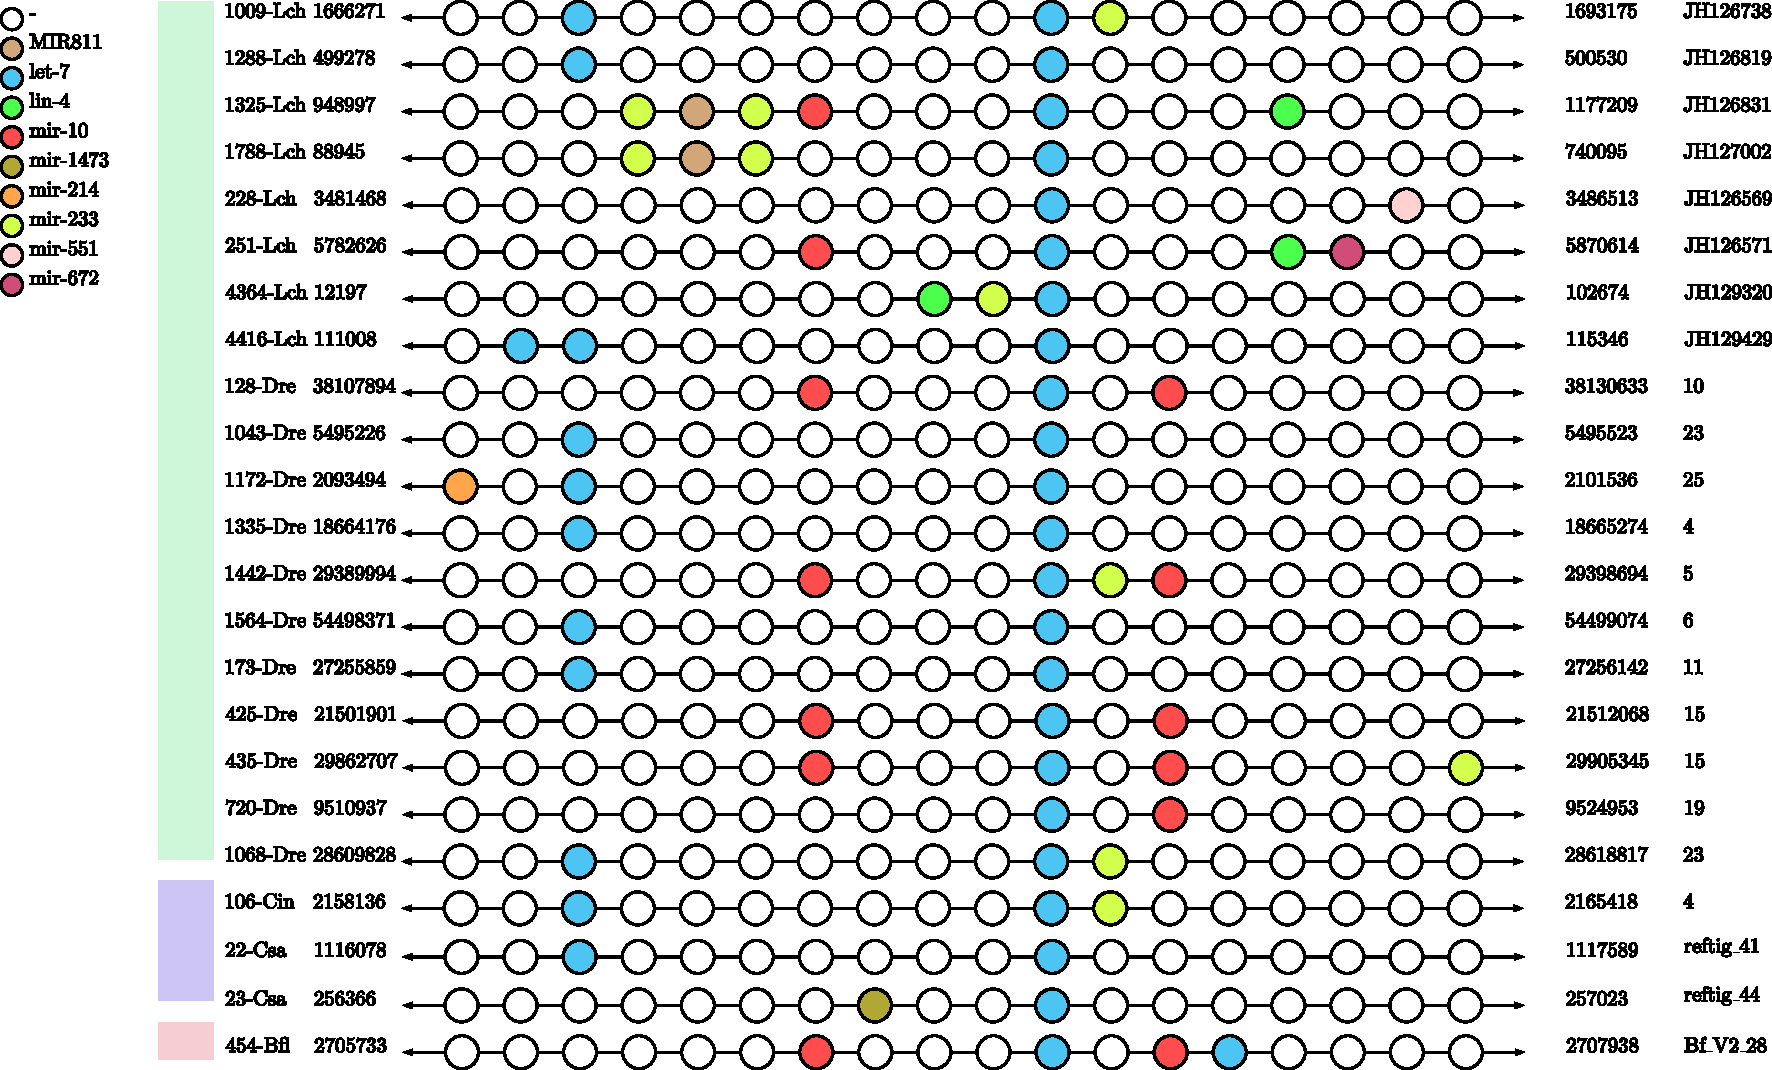
\includegraphics[height=9 cm]{Cluster_images/let-7_101_128}
        \caption{let-7}
\label{let-7}

    \end{subfigure}
    \\
    \begin{subfigure}[t]{0.45\textwidth}
        \centering
        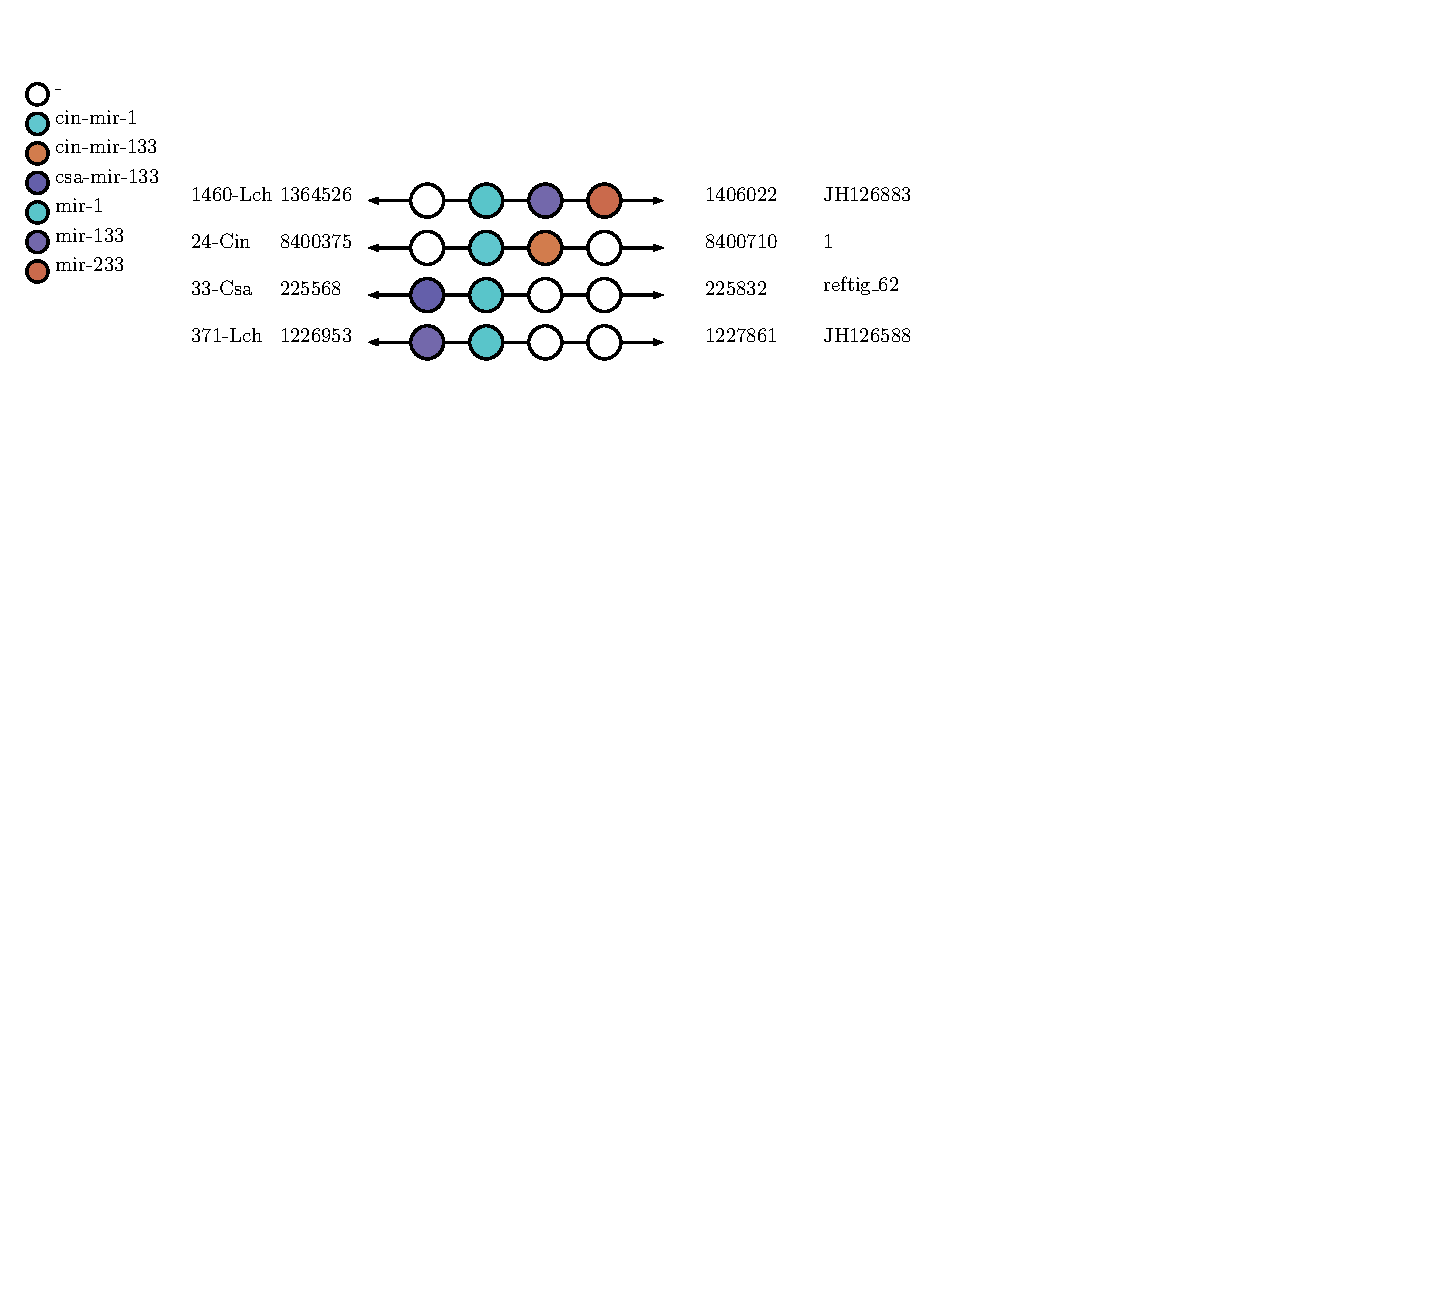
\includegraphics[height=1.2 cm]{Cluster_images/mir-1_119_33}
        \caption{mir-1/mir-133}
\label{mir-1/mir-133}

     \end{subfigure}
        ~
     \\
    \begin{subfigure}[t]{0.45\textwidth}
        \centering
        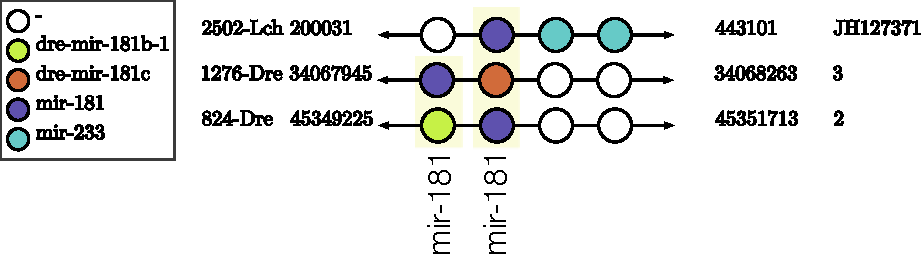
\includegraphics[height=1.2 cm]{Cluster_images/mir-181_105_2502}
        \caption{mir-181}
 \label{mir-181}
       \end{subfigure}
        ~
         \begin{subfigure}[t]{0.45\textwidth}
        \centering
        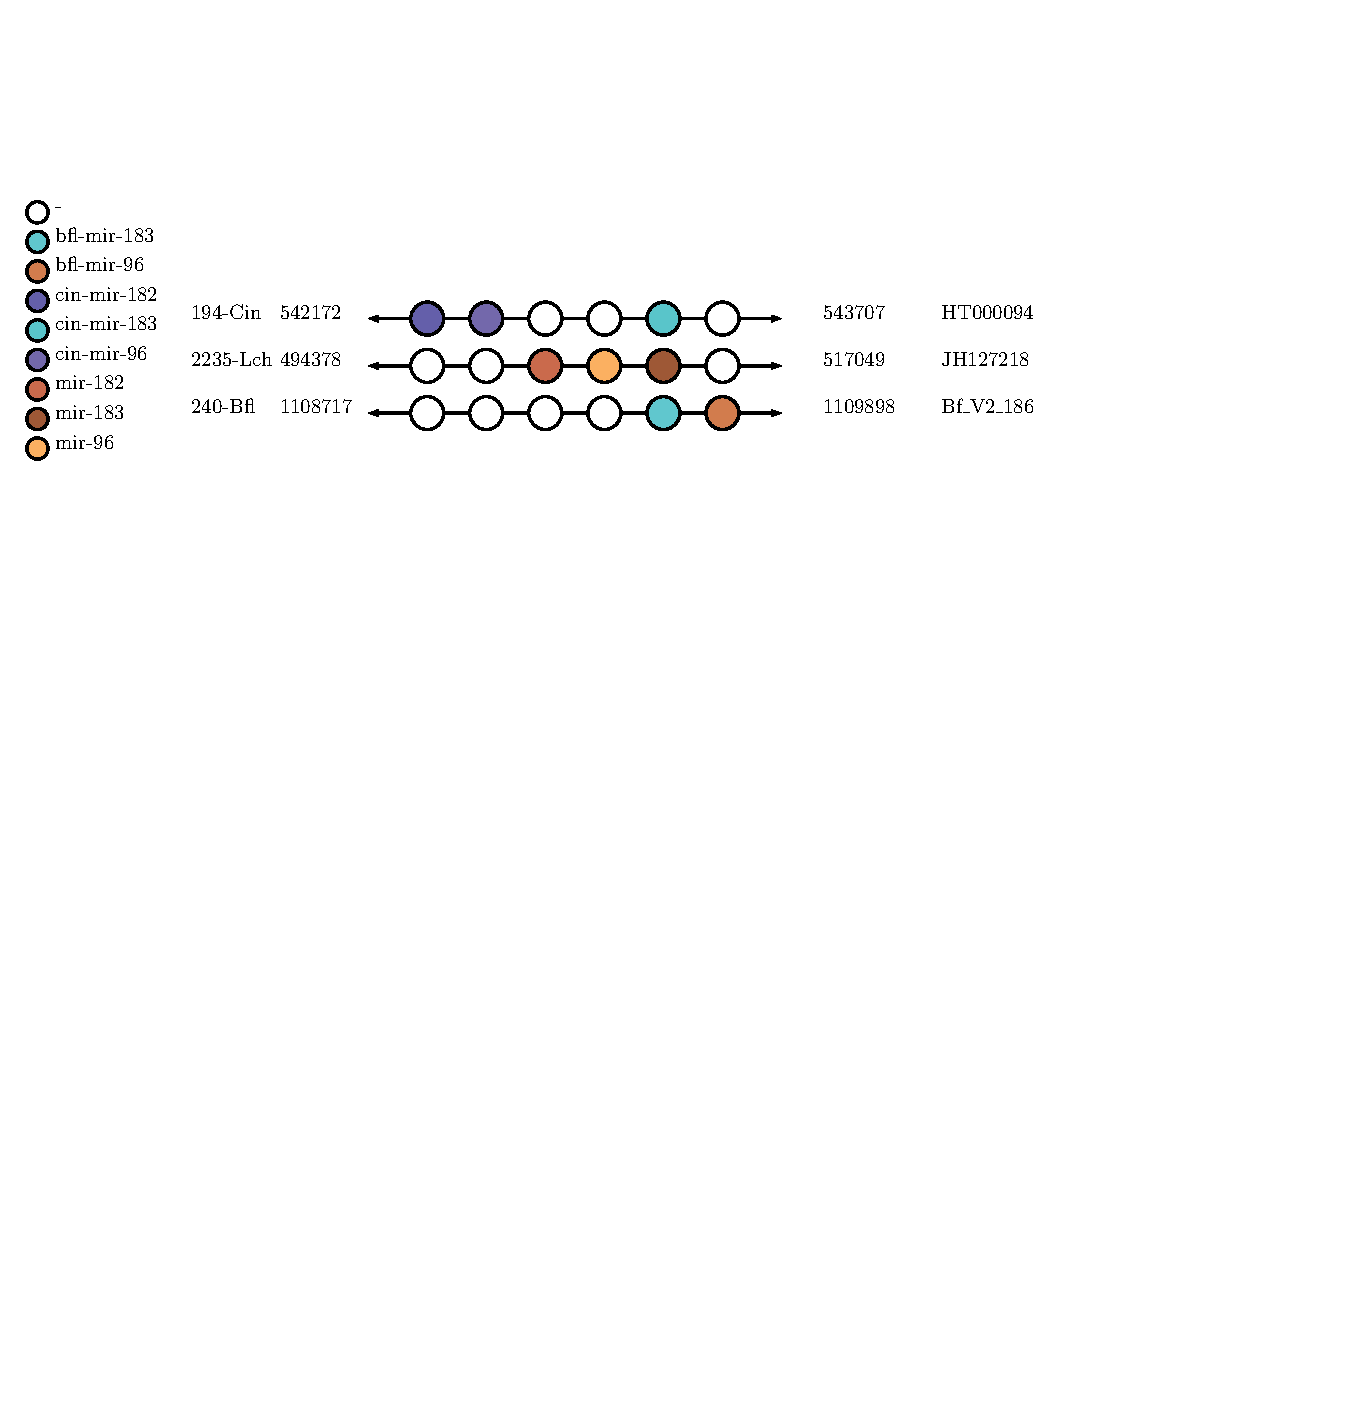
\includegraphics[height=1.2 cm]{Cluster_images/mir-183_132_240}
        \caption{mir-183}
 \label{mir-183}
    \end{subfigure}
    \\
    \begin{subfigure}[t]{0.45\textwidth}
        \centering
        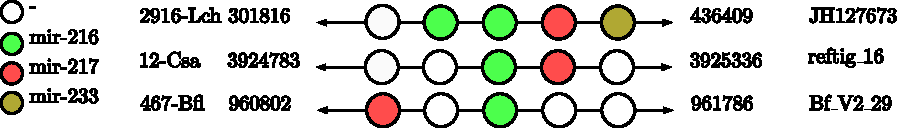
\includegraphics[height=1.2 cm]{Cluster_images/mir-216_126_467}
        \caption{mir-216/mir-217}
 \label{mir-216/mir-217}       
\end{subfigure}
     \\
    \begin{subfigure}[t]{0.45\textwidth}
        \centering
        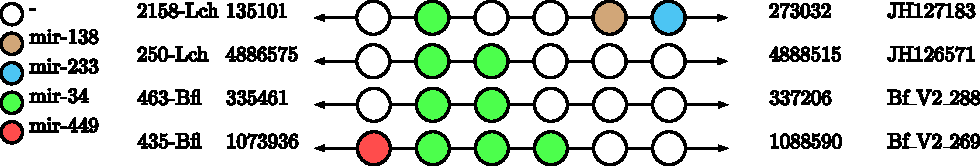
\includegraphics[height=1.2 cm]{Cluster_images/mir-34_11A_435}
        \caption{mir-34}
 \label{mir-34}       
\end{subfigure}
        ~
         \begin{subfigure}[t]{0.45\textwidth}
        \centering
        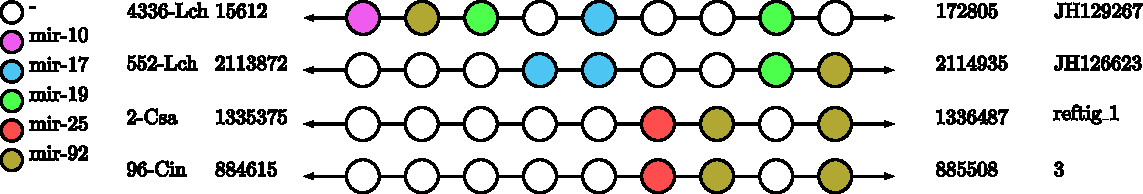
\includegraphics[height=1.2 cm]{Cluster_images/mir-92_281_4336}
        \caption{mir-92}
\label{mir-92}
    \end{subfigure}
    \\
    \caption{Multiple alignments of miRNA's clusters. \textbf{Prot}: Protostomata, \textbf{Brfl}: \textit{B. floridae}, 
\textbf{Oidi}: \textit{O. dioica}, \textbf{Dvex}: \textit{D. vexillum}, 
\textbf{Ciin}: \textit{C. intestinalis}, \textbf{Cisa}: \textit{C. savignyi}, 
\textbf{Ciro}: \textit{C. robusta}, \textbf{Sath}: \textit{S. thompsoni}, 
\textbf{Mata}: \textit{M. oculata}, \textbf{Mlta}: \textit{M. occulta}, 
\textbf{Mlis}: \textit{M. occidentalis}, \textbf{Bosc}: \textit{B. schlosseri}, 
\textbf{Haro}: \textit{H. roretzi}, \textbf{Pema}: \textit{P. marinus}, 
\textbf{Dare}: \textit{D. rerio}, \textbf{Lach}: \textit{L. chalumnae}, 
\textbf{Xetr}: \textit{X. tropicalis} and \textbf{Anca}: \textit{A. 
carolinensis}.} \label{altclusters}
\end{figure}









\newpage











\begin{longtable}{p{1 cm}p{2.3 cm}p{2 cm}p{2 cm}p{2 cm}p{1.5 cm}p{1.8 cm}p{3 cm}}
\textbf{Clade}&\textbf{Specie} & \textbf{Chr} & \textbf{Start} & \textbf{End} & \textbf{Size(Mb)} & \textbf{No. miRNAs} & \textbf{Elements} \\
\toprule
C & \textit{B. floridae} & Bf\_V2\_118 & $216744$ & $220351$ & $3607$ & $5$ & bfl-mir-4869, bfl-mir-4857, bfl-mir-4862, bfl-mir-4856b, bfl-mir-4856a \\
T & \textit{O. dioica} & scaffold\_3 & $2222857$ & $2223714$ & $857$ & $6$ & odi-mir-1497e, odi-mir-1497d-2, odi-mir-1497d-1, odi-mir-1497c, odi-mir-1497b, odi-mir-1497a \\
T & \textit{B. schlosseri} & chrUn & $40003$ & $41320$ & $1317$ & $2$ & mir-233, mir-10 \\
T & \textit{C. intestinalis} & $7$ & $4153284$ & $4156782$ & $3498$ & $23$ & cin-mir-4006d, cin-mir-4006c, cin-mir-4001b-2, cin-mir-4000i, cin-mir-4006g, cin-mir-4001e, cin-mir-4001d, cin-mir-4000g, cin-mir-4006f, cin-mir-4006b, cin-mir-4001b-1, cin-mir-4000c, cin-mir-4006e, cin-mir-4000b-2, cin-mir-4001a-1, cin-mir-4000b-1, cin-mir-4002, cin-mir-4000d, cin-mir-4001h, cin-mir-4000a-2, cin-mir-4006a-2, cin-mir-4006a-3, cin-mir-4006a-1 \\
T & \textit{C. savignyi} & reftig\_16 & $3924783$ & $3925336$ & $553$ & $3$ & csa-mir-216b, csa-mir-216a, csa-mir-217 \\
T & \textit{C. savignyi} & reftig\_1 & $1335375$ & $1336487$ & $1112$ & $3$ & csa-mir-92b, csa-mir-92c, csa-mir-92a \\
V & \textit{D. rerio} & $4$ & $28738556$ & $28754891$ & $16335$ & $60$ &  \small{dre-mir-430a-18, dre-mir-430c-18, dre-mir-430b-4, dre-mir-430a-15, dre-mir-430c-18, dre-mir-430b-5, dre-mir-430a-10, dre-mir-430c-18, dre-mir-430b-5, dre-mir-430a-15, dre-mir-430c-18, dre-mir-430b-3, dre-mir-430a-10, dre-mir-430c-18, dre-mir-430b-8, dre-mir-430a-15, dre-mir-430c-18, dre-mir-430b-5, dre-mir-430a-17, miR-430, dre-mir-430b-20, dre-mir-430a-10, dre-mir-430c-18, dre-mir-430b-5, dre-mir-430i-3, dre-mir-430c-18, dre-mir-430b-3, dre-mir-430a-10, dre-mir-430c-18, dre-mir-430b-8, dre-mir-430a-11, dre-mir-430c-18, dre-mir-430b-5, dre-mir-430i-3, dre-mir-430c-18, dre-mir-430b-19, dre-mir-430a-10, dre-mir-430c-18, dre-mir-430b-5, dre-mir-430a-17, miR-430, dre-mir-430b-20, dre-mir-430a-10, dre-mir-430c-18, dre-mir-430b-5, dre-mir-430i-3, dre-mir-430c-18, dre-mir-430b-19, dre-mir-430a-10, dre-mir-430c-18, dre-mir-430b-5, dre-mir-430a-15, dre-mir-430c-18, dre-mir-430b-3, dre-mir-430a-10, dre-mir-430c-18, dre-mir-430b-8, dre-mir-430a-15, dre-mir-430c-18, dre-mir-430b-5} \\
V & \textit{L. chalumnae} & JH126646.1 & $1529355$ & $1882777$ & $353422$ & $7$ & mir-233, mir-233, mir-233, mir-598, mir-672, MIR535, mir-233 \\
\bottomrule
\caption{Details of biggest miRNA cluster for chordate species}
\label{tab:detailBigClusters}
\end{longtable}
  
\begin{figure}[ht]
\centering
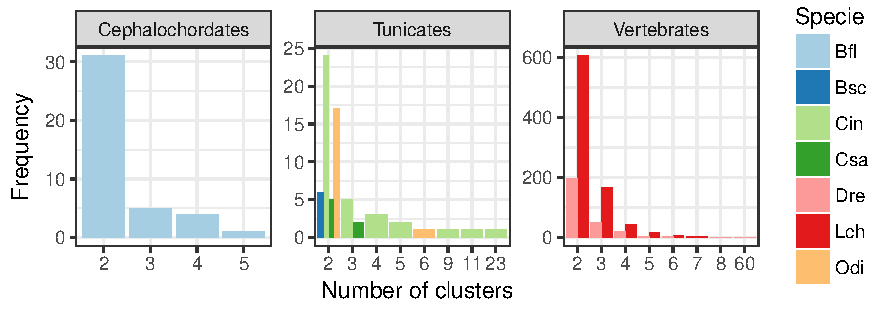
\includegraphics[scale=1]{Cluster_images/cluster_number.pdf} \\ 
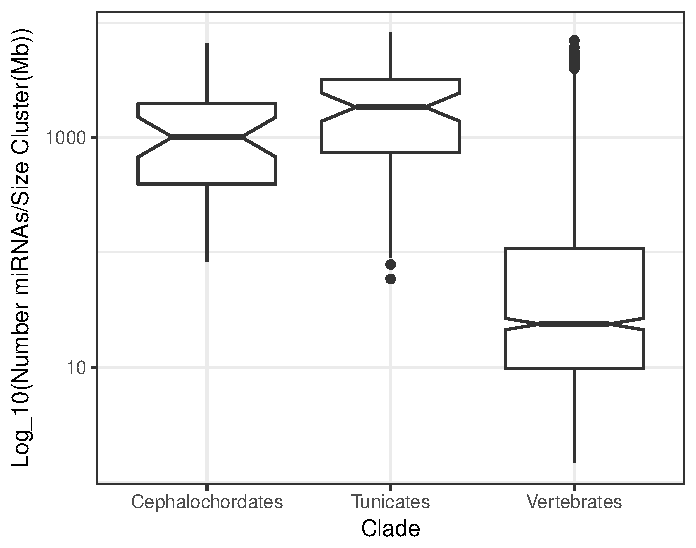
\includegraphics[scale=0.7]{Cluster_images/density.pdf} 
\caption{Analysis of the distribution, size and number's of cluster along chordate species.}
\label{fig:sizeCluster}
\end{figure}

\newpage


\subsubsection*{Results}


Applying the last strategy to detect miRNA's clusters granted the option to study the conserved elements along chordate's genomes. As shown in Figure \ref{fig:sizeCluster}, directly with the location form those miRNA elements have been possible to identify the number and the length of those identified regions along all the studied genomes. In this case, the cluster that contains the greatest number of miRNAs elements ($60$) is located on \textit{D. rerio} genome: \texttt{Chromosome $4$:$28738556$-$28754891$}, for tunicates on \textit{C. intestinalis}: \texttt{Chromosome $7$:$4153284$-$4156782$} with $23$ elements, and in \textit{B. floridae}: \texttt{Bf\_V2\_118: $216744$-$220351$} only $5$ miRNAs have been detected (for further details Table \ref{tab:detailBigClusters} describe the miRNAs families located inside the largest clusters for each specie). Additionally, is more frequent to found clusters that contain $2$ miRNAs families, but is also important to know that the relation between the number of miRNAs inside a cluster and the cluster's length is higher on tunicates and cephalochordates in comparison to vertebrates, it means that inside the identified clusters along vertebrates the miRNAs elements are more distant between them. 


Comparison between miRNA clusters have been calculated in order to access to the 
most conserved set of miRNA families inside chordate's clusters. As a result, the following miRNAs families were identified being part of specific clusters regions: let-7, mir-1, 
MIR1122, mir-130, mir-132, mir-133, mir-135, mir-146, mir-15, mir-17, mir-181, 
mir-183, MIR1846, mir-186, mir-19, mir-193, mir-216, mir-219, mir-23, mir-24, 
mir-242, mir-25, mir-27, mir-286, mir-29, mir-2985-2, mir-30, mir-34, mir-395, 
mir-454, mir-489, MIR535, mir-8, mir-9 (Figure \ref{altclusters}).



\newpage
\bibliographystyle{plain}
\bibliography{tuni}

\end{document}


%%% Local Variables:
%%% mode: latex
%%% TeX-PDF-mode: t
%%% End:
